\documentclass[journal,twoside,web]{ieeecolor}
\usepackage{tmi}
\usepackage{cite}
\usepackage{amsmath,amssymb,amsfonts}
\usepackage{algorithmic}
\usepackage{graphicx}
\usepackage{textcomp}
\usepackage{epstopdf}
\usepackage{multirow}
\usepackage{caption}
\usepackage{subfigure}
\usepackage{booktabs}
\let\labelindent\relax
\usepackage{enumitem}
\usepackage[table]{xcolor}
\usepackage{tabularx,ragged2e}

\usepackage{algorithm}
\usepackage{algorithmic}

\def\BibTeX{{\rm B\kern-.05em{\sc i\kern-.025em b}\kern-.08em
    T\kern-.1667em\lower.7ex\hbox{E}\kern-.125emX}}
\markboth{submitted to IEEE Transactions on Medical Imaging}
{Author \MakeLowercase{\textit{Zhang et al.}}:Generator Versus Segmentor: Pseudo-healthy Synthesis}
\begin{document}
\title{Generator Versus Segmentor: Pseudo-healthy Synthesis}
%\title{Teaching by Books: \\ Semi-supervised Medical Image Segmentation From Mixed Supervision}
\author{Yunlong Zhang, Xin Lin, Yihong Zhuang, Liyan Sun, Yue Huang, Xinghao Ding, Guisheng Wang, Yizhou Yu, \IEEEmembership{Fellow, IEEE} and Lin Yang
\thanks{The work is supported in part by National Key Research and Development Program of China (No. 2019YFC0118104), in part of ZheJiang Province Key Research Development Program (No. 2020C03073), in part by National Natural Science Foundation of China under Grants 81671766, 61971369, U19B2031, U1605252, 61671309, in part by Open Fund of Science and Technology on Automatic Target Recognition Laboratory 6142503190202, in part by Fundamental Research Funds for the Central Universities 20720180059, 20720190116, 20720200003, and in part by Tencent Open Fund.}
\thanks{Yunlong Zhang, Xin Lin, Yihong Zhuang, Liyan Sun, Yue Huang, and Xinghao Ding are with the
School of Informatics, Xiamen University, Xiamen 361005, China (e-mail:
dxh@xmu.edu.cn). }
\thanks{Guisheng Wang is with the Department of Radiology, the Third Medical Centre, Chinese PLA General Hospital, Beijing, China
(e-mail: wanggs1996@tom.com)}
\thanks{Yizhou Yu is with the Deepwise AI Laboratory, Beijing 100125, China
(e-mail: yizhouy@acm.org)}
\thanks{Lin Yang is with the School of Engineering, Westlake University, Hangzhou 310012, China
	(e-mail: yanglin@westlake.edu.cn)}
}

\maketitle

\begin{abstract}
Synthesizing a subject-specific pathology-free image from a pathological one is valuable for algorithm development and clinical practice. In recent years, approaches based on Generative Adversarial Network (GAN) were presented and achieved promising results. In this paper, we discover that the discriminator in GAN cannot accurately identify the lesions in images and further hampers from generating admirable pseudo-healthy images. To address this problem, we creatively introduce the segmentor as the discriminator. It is able to accurately locate the lesions and contributes to improving the visual quality of pseudo-healthy images. Then, we develop an image enhancement technique by adding the residues between original and synthetic images into the former and utilize this technique to cope with the low contrast problem existing in the medical image segmentation. Furthermore, in response to the problem of lacking proper metrics to measure how healthy the synthetic images look, we propose a stable and reliable metric by fully utilizing two attributes of label noise. Experiments on public dataset BraTS demonstrate that the proposed method substantially outperforms state-of-the-art methods. Especially, only utilizing 30 percent of training data, our method achieves comparable performance to the existing methods. Furthermore, we also certify the effectiveness of our method on dataset LiTS.
\end{abstract}

\begin{IEEEkeywords}
Medical Image Synthesis, Medical Image Segmentation, Adversarial Training, Image Enhancement, Label Noise
\end{IEEEkeywords}

\section{Introduction}
\label{sec:introduction}


\begin{figure}
	\centering
	\subfigure[Input]{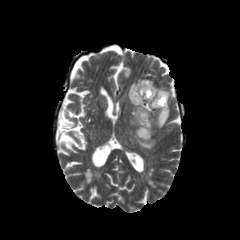
\includegraphics[width=0.24\columnwidth]{./figs/340_original.jpg}\label{fig11}}
	\subfigure[Segmentor]{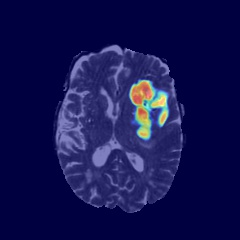
\includegraphics[width=0.24\columnwidth]{./figs/340_seg_grad_cam.jpg}\label{fig12}}
	\subfigure[Classifier]{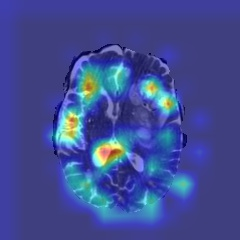
\includegraphics[width=0.24\columnwidth]{./figs/340_grad_cam.jpg}\label{fig13}}
	\subfigure[Label]{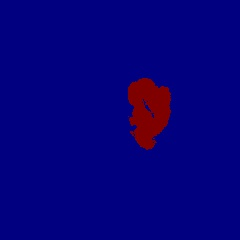
\includegraphics[width=0.24\columnwidth]{./figs/340_label.jpg}\label{fig14}}\\
	\subfigure[Input]{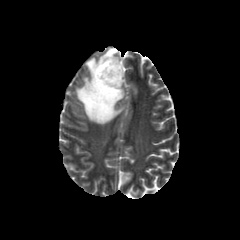
\includegraphics[width=0.24\columnwidth]{./figs/100_original.jpg}\label{fig15}}
	\subfigure[Segmentor]{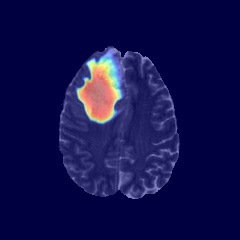
\includegraphics[width=0.24\columnwidth]{./figs/100_seg_grad_cam.jpg}\label{fig16}}
	\subfigure[Classifier]{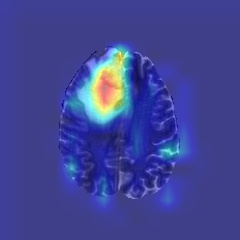
\includegraphics[width=0.24\columnwidth]{./figs/100_grad_cam.jpg}\label{fig17}}
	\subfigure[Label]{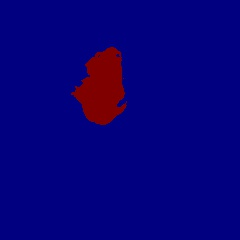
\includegraphics[width=0.24\columnwidth]{./figs/100_label.jpg}\label{fig18}}
	\caption{'Visual explanations' for the classifier and segmentor. (a-d) represent one example. They respectively are one input, class activation maps generated by Grad-CAM \cite{selvaraju2017grad} and Seg-Grad-CAM \cite{vinogradova2020towards}, and tumor annotation. (e-h) are corresponding images for another example.
	}\label{fig1}
\end{figure}

Pseudo-healthy synthesis is defined as synthesizing a subject-specific pathology-free image from a pathological one \cite{bowles2016pseudo,xia2020pseudo}. Generating such images has been proven to be valuable for a variety of medical image analysis tasks \cite{xia2020pseudo}, such as segmentation \cite{bowles2017brain,ye2013modality,sun2020adversarial,andermatt2018pathology,bowles2016pseudo}, detection \cite{tsunoda2014pseudo}, and providing additional diagnostic information for pathological analysis \cite{baumgartner2018visual,sun2020adversarial}. In clinical applications, a perfect pseudo-healthy image should maintain both healthiness (i.e., pathological regions are in harmony with healthy ones in synthetic images) and subject identity (i.e., belonging to the same subject as the input). Note that both of them are essential and indispensable. The importance of the former is self-explanatory, and the latter is also considerable since generating another healthy image is meaningless.

Recently, several GAN-based methods \cite{baumgartner2018visual,sun2020adversarial,xia2020pseudo} were presented to tackle the problem of pseudo-healthy synthesis and achieved promising results. The key components in these methods are a generator and a discriminator. The former is trained to translate pathological images into corresponding healthy-looking ones, whereas the latter competes against the former and aims to differentiate synthetic and healthy images by a two-way classifier. However, choosing the classifier as the discriminator has the shortcoming of not being able to accurately locate the lesions, which are described in detail as follows. First, the classifier makes decisions based on not only pathological regions but also heterogeneous healthy ones (e.g., the 'tumor' explanation highlights both pathological regions and heterogeneous pixels in healthy regions in Figure \ref{fig13}), which enforces the generator to modify the highlighted regions that affirm classification decision. Furthermore, the subject identity will be erased since the whole synthetic image deviates from the original one. Second, the classifier makes decisions based on the pixels with the most evident pathological signal. That being said, only a part of pathological pixels with the most evident signals are enough to assure the correct classification (e.g., the 'tumor' explanation highlights the core pixels in pathological regions in Figure \ref{fig17}). Hence, the remaining pixels with weaker pathological signals are not changed towards healthy appearances, which eventually harms the healthiness of synthetic images.

To overcome the aforesaid shortcomings, we choose the segmentor as the discriminator. In comparison with the classifier, the segmentor identifies pathological regions more accurately (the 'tumor' explanation accurately highlights tumor regions in Figure \ref{fig12} and \ref{fig16}). Therefore, the subject identity and healthiness can be simultaneously maintained by respectively keeping the healthy pixels and transforming the pathological ones. The former is implemented by a visual residual loss, and the latter is achieved by the adversarial training between the generator and the segmentor.

During the process of adversarial training, pathological pixels in the synthetic images are gradually close to healthy-looking ones. These healthy-like pixels should be labeled as 'no tumor' but be falsely labeled as 'tumor' when training the segmentor, which eventually results in the poor generalization performance of the segmentor. To address this issue, we propose a difference-aware loss, which improves the generalization ability of the segmentor by muting those confusingly healthy-looking pixels. 

%It is well-known that the adversarial training between the generator and classifier is notorious for difficult optimization due to the challenge of attaining Nash equilibrium of a non-convex min-max game in high-dimensions \cite{barnett2018convergence,chu2020smoothness,kodali2017convergence}. By contrast, the adversarial training between the generator and the segmentor can effectively reduce the dimensionality of the input space (i.e., the dimension of the entire image for the classifier v.s. the dimension of the receptive field for the segmentor), which alleviates the optimization problem in the adversarial training. Benefiting from this, our method has lower requirements for large quantity of training samples. So it can be better applied in practice.

%We develop the proposed method to enhance contrast between lesions and healthy tissues. It is well-known that low-contrast medical images make tissue segmentation a challenging problem. Image enhancement, as an effective pre-processing technique, has been broadly applied in medical image segmentation tasks \cite{vasuki2017survey}. 

Besides providing subjectively pathology-free results, the synthetic images generated by our method also contribute to the segmentation task. It is well-known that the low contrast is a nasty nature of medical images, which may result in the difficulty in distinguishing different anatomies. Since our method can effectively disentangle pathological and healthy signals in the image space, we design an image enhancement technique of highlighting lesions by simply adding the extracted pathological signals into original images and then apply this technique to enhancing the contrast between lesions and normal tissues and further improving segmentation performance. 

Another major barrier in pseudo-healthy synthesis is lacking a good quantitative metric for measuring 'healthiness'. Recently, Xia et al. \cite{xia2020pseudo} proposed a metric by pre-training a segmentor on pathological images and then estimating the remaining pathological signal on synthetic outputs. The remaining pathological signal indirectly reflects the healthiness, and the lower one represents the better healthiness. However, model selection drastically impacts the final results, and so it achieves lower repeatability and reproducibility. Worse, it is vulnerable and unreliable when appearing artifacts far away from both pathological and healthy regions in the distributional space. On the other hand, subjective assessment is viewed as the gold standard to ultimately determine the healthiness \cite{xia2020pseudo}. However, it is time-consuming and costly, while being subject to inter- and intra-observer variability, and hence also deviates from the reproducibility. Inspired by the study of label noise that fitting incorrect labels requires more time \cite{zhang2016understanding} and the higher learning rate hampers the memorization of false labels, we propose a stable and reliable metric by estimating the convergence speed to measure healthiness.

To provide evidence for these claims, we conduct an extensive evaluation on the BraTS dataset \cite{bakas2017advancing,menze2014multimodal,bakas2018identifying}.  Furthermore, we also present a part of results on the LiTS \cite{bilic2019liver} that indicate that our method has the potential to expand into different modalities and organs. 

The rest of this paper is organized as follows. In Section \ref{sec:RelatedWorks}, we review the literature related to pseudo-healthy synthesis and some representative adversarial methods. In Section \ref{sec:Methods}, we present the proposed GVS. In Section \ref{sec4}, we propose a new metric, A-Dice, to measure 'Healthiness' and highlight its advantages by experiments and analysis. In Section \ref{sec5}, we conduct extensive experiments to validate the effectiveness of our proposed method. Section \ref{sec6} concludes the full paper and further discusses the limitations of our method and future work.

\begin{figure*}[htbp]
	\centering
	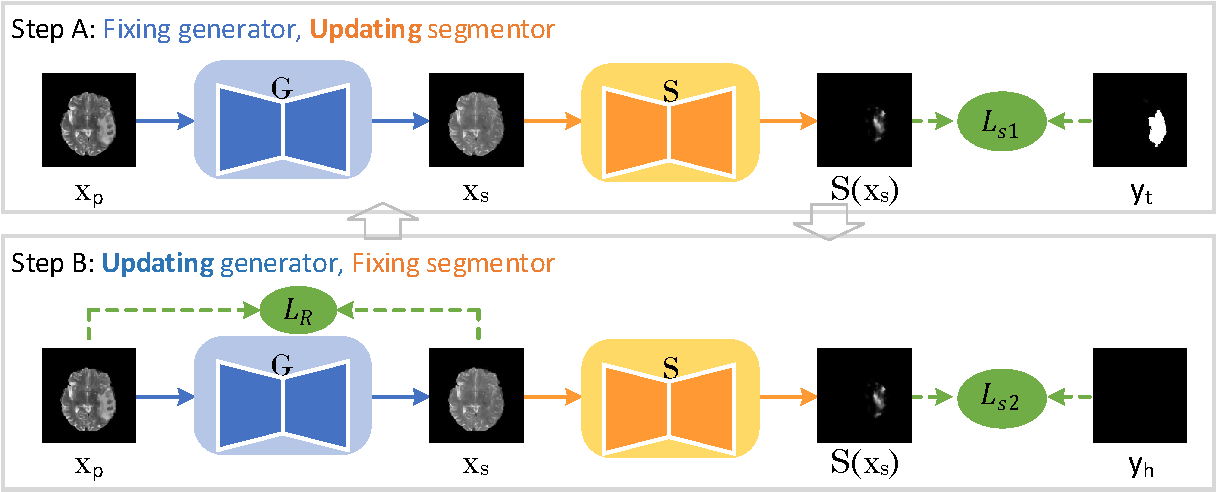
\includegraphics[width=\textwidth]{./figs/framework.pdf}
	\caption{Training workflow. We use an encoder-decoder architecture for the generator $\mathbf{G}$ and a U-Net architecture for the segmentor $\mathbf{S}$. The model is optimized by iteratively alternating Step A and Step B. In Step A, we fix the generator $\mathbf{G}$ and update the segmentor $\mathbf{S}$ with $L_{s1}$. In Step B, we fix the segmentor $\mathbf{S}$ and update  the generator $\mathbf{G}$ with $L_{s2}+L_R$.}
	\label{fig2}
\end{figure*}

\section{Related Works}
\label{sec:RelatedWorks}
\subsection{Pseudo-healthy synthesis}
Recently, pseudo-healthy synthesis attracted much attention in medical image analysis community because of its potential for downstream tasks \cite{bowles2017brain,ye2013modality,sun2020adversarial,andermatt2018pathology,tsunoda2014pseudo,chen2018unsupervised,baumgartner2018visual,xia2020pseudo}. We divide the related works into two main categories,  pathology-deficiency (i.e., only containing healthy images in the training phase) \cite{chen2018unsupervised,sato2018primitive,schlegl2019f} and pathology-sufficiency based methods (i.e., possessing plenty of pathological and healthy images in the training phase) \cite{baumgartner2018visual,sun2020adversarial,xia2020pseudo}.

Pathology-deficiency based methods \cite{baur2018deep,zimmerer2019unsupervised,zimmerer2018context,chen2018unsupervised,pawlowski2018unsupervised,Baur2020ScaleSpaceAF,Baur2020SteGANomalyIC,Nguyen2020UnsupervisedRA} were always closely associated with unsupervised anomaly detection/segmentation \cite{baur2021autoencoders}, which aimed to learn normative distribution by learning to compress and recover healthy anatomy in the training phase. In the subsequent testing stage, pathological images were first compressed to the latent space. These methods assumed that obtained latent representations were close to counterparts of pseudo-healthy images. Based on this assumption, pseudo-healthy images were reconstructed from latent representations. Actually, the assumptions of these methods were over ideal \cite{chen2018unsupervised,schlegl2019f}. Actually, the healthiness and subject identity were not guaranteed due to the inability to obtain the optimal latent representations corresponding to pseudo-healthy images. 

Pathology-sufficiency based methods \cite{baumgartner2018visual,sun2020adversarial,xia2020pseudo} tackled pseudo-healthy synthesis from another way. These methods introduced pathological images alongside corresponding image-level \cite{baumgartner2018visual} or pixel-level \cite{sun2020adversarial,xia2020pseudo} pathological annotations in the training phase.  Baumgartner et al. \cite{baumgartner2018visual} proposed a basic GAN-based scheme, which was composed of a generator and a discriminator. The generator is trained to fool the discriminator and keep the reconstructed images close to the original ones and the discriminator aims to differentiate the synthetic images from the unpaired healthy ones. Note that this method only used the image-level annotations and cannot accurately translate pathological pixels and keep healthy ones. To alleviate this issue, PHS-GAN \cite{xia2020pseudo} and ANT-GAN \cite{sun2020adversarial} introduced the pixel-level annotations. Meanwhile, both of them were the variants of Cycle-GAN \cite{zhu2017unpaired}. Concretely, PHS-GAN considered the one-to-many problem and disentangled the information of pathology from what seems to be healthy, and pixel-level labels were used to extract the location and shape of the pathology. ANT-GAN proposed two improvements in the process of applying Cycle-GAN to pseudo-healthy synthesis. The first one is the shortcut to simplify the optimization,  and the second one is the masked L2 loss to better preserve the normal regions.

Our method is identical with the work by Sun et al. \cite{sun2020adversarial} and Xia et al. \cite{xia2020pseudo} in the experimental setting,  but our motivation is significantly different from them. They tried to translate pathological images into healthy-looking appearances learned from massive healthy images. In comparison, our method further explicitly utilized the difference information containing in the appearance differences between healthy and pathological regions and tried to generate pathology-free images by making up such differences until achieving harmony between them. 

\subsection{Adversarial training}
The idea of adopting the segmentor as the discriminator is inspired by the extensive applications of adversarial training \cite{goodfellow2014generative}. The discriminator of the original GAN was used to differentiate true or counterfeit images. In domain adaptation, DANN \cite{ganin2016domain}  adopted a discriminator to distinguish the source or target domains. In the research on the adversarial attack,  the discriminator is a classifier to sort an example into corresponding class \cite{goodfellow2014explaining,miyato2018virtual}. In image translation tasks, the discriminator also is a classifier to detect the high-level structured difference between translations and labels \cite{isola2017image,zhu2017unpaired}.  Recently, Naveen et al. \cite{minderer2020automatic} applied adversarial training into self-supervised learning and adopted a classifier as the discriminator to predict pretext labels. In comparison with related work using diverse classifiers as discriminators, we further develop the paradigm of adversarial training and extend the discriminator to pixel-level dense prediction task.



\section{Methods}
\label{sec:Methods}
In this section, the proposed GVS method for pathology-sufficiency pseudo-healthy synthesis with pixel-level labeling is introduced. Assume a set of pathological images $\{x_p\}$ with their pixel-level lesion annotations $\{y_t\}$ are given. Our goal is to train a generator $\mathbf{G}$ that can translate the pathological image $x_p$ into corresponding synthetic one $x_s$ with the superior healthiness and subject identity.

\begin{figure*}
	\centering
	\includegraphics[width=\textwidth]{./figs/wce.pdf}
	\caption{(a) Framework of the pixel-level weighted cross-entropy loss. (b) The blue, yellow, green, and red boxes denote the pathological image, synthetic image, segmentation predictions, and lesion annotations, respectively.
	}\label{fig4}
\end{figure*}

\subsection{Basic GVS flowchart}
\label{subsection:flowchart}
The training workflow of the proposed GVS is shown in Figure \ref{fig2}. The generator gradually synthesizes pseudo healthy images by iteratively alternating Steps A and B. The specific steps are described as follows.

\noindent\textbf{Step A.} As shown in the Step A of Figure \ref{fig2}, we fix the generator $\mathbf{G}$ and update the segmentor $\mathbf{S}$ to segment the lesions in the synthetic images. The loss is defined as:
\begin{equation}
	\mathcal{L}_{s1} = \mathcal{L}_{ce}(\mathbf{S}(x_s)), y_t),
\end{equation} 
where $L_{ce}$ denotes the cross-entropy loss.

\noindent\textbf{Step B.} In this step, we fix the segmentor $\mathbf{S}$ and update the generator $\mathbf{G}$, aiming to remove the lesions and preserve the subject identity of pathological images. 
On the one hand, it is expected that generator $\mathbf{G}$ can synthesize pseudo healthy images that do not contain lesions. Therefore, an adversarial loss is utilized,
\begin{equation}\label{eq2}
	\mathcal{L}_{s2} = \mathcal{L}_{ce}(\mathbf{S}(\mathbf{G}(x_p))), y_h),
\end{equation} 
where $y_h$ denotes the zero matrix with the same size as $y_t$. To deceive the segmentor, the generator further compensates the distributional difference between pathological and healthy regions. 
On the other hand, the synthetic images should be consistent with the pathological ones visually. Hence, the residual loss proposed in existing pseudo-healthy synthesis method \cite{sun2020adversarial} is used:
\begin{equation}\label{eq3}
	\mathcal{L}_R = \mathcal{L}_{mse}(x_p,  \mathbf{G}(x_p)),
\end{equation} 
where $\mathcal{L}_{mse}$ denotes pixel-wise $\mathcal{L}_2$ loss.  The total training loss of  $\mathbf{G}$ is:
\begin{equation}
	\mathcal{L}_{G} = \mathcal{L}_{s2} + \lambda \mathcal{L}_R,
\end{equation} 
where $\lambda$ denotes a hyperparameter that trades off the healthiness against identity, and $\lambda > 0$.
 
%The adversarial relationship between segmentor $\mathbf{S}$ and generator $\mathbf{G}$ during the iterative training of them completes each other in turn. $\mathbf{S}$ learns to fit the pixel-level healthy distribution when meeting $\mathbf{G}$ generates various anomalies to deceive him. In turn,  $\mathbf{G}$ can synthesize better healthy-like appearance in pathological regions.

During the iterative training, the segmentor $\mathbf{S}$ and the generator $\mathbf{G}$ compete with each other. The segmentor $\mathbf{S}$ tried to detect the differences between normal and pathological regions, whereas the generator $\mathbf{G}$ tried to make up them. Eventually, $\mathbf{G}$ harmonizes the pathological and normal regions and synthesizes healthy-like images.

%\begin{figure*}[htbp]
%	\centering
%	\includegraphics[width=\textwidth]{wce.pdf}
%	\caption{(a) Framework of the pixel-level weighted cross-entropy loss. (b) The blue, yellow, green, and red boxes denote the pathological image, synthetic image, segmentation predictions, and lesion annotations, respectively.}
%	\label{fig3}
%\end{figure*}




%\subsection{Improved residual loss}
%\label{subsection:residual}
%This section further discusses the reasonableness of Eq. \ref{eq3} and proposed an improved residual loss (IRL). First, considering the subject identity, keeping consistency between pathological and synthetic images is reasonable and necessary for the normal region. Hence, we still set a visually consistent loss between them. Then, for the pathological region, the $\mathcal{L}_R$ closes the pathological and synthetic images visually. However, it is contradictory to remove lesions and keep pixel values for pathological pixels. To overcome this contradiction, we assume the pixel values of potential normal tissue for pathological region are close to the normal tissue in the same pathological image. Hence, we introduce a constraint that closes the visual residue between pixel values of pathological region and average value of the normal tissue in the same pathological image. To sum up, we proposed the improved residual loss as follows,
%
%\begin{equation}
%	\begin{aligned}
%		\mathcal{L}_{R+} = \mathcal{L}_{mse}((1-y_t)\odot x_p,(1-y_t)\odot  \mathbf{G}(x_p))\\
%		 + \lambda_1 \mathcal{L}_{mse}(y_t\odot \overline x_{pn},y_t\odot \mathbf{G}(x_p)),
%	\end{aligned}
%\end{equation}
%where $\odot$ represents the pixel-wise multiplication, and $\overline x_{pn}$ denotes a matrix filled with the average value of normal tissue in image $x_p$ and has the same size as $x_p$; $\lambda_1$ denotes a hyperparameter that controls the power of consistent constrain in the pathological region, and $0<\lambda_1<1$ since the pixel values of potential normal tissue close but not equal to the average value of normal tissue.



\subsection{Training a segmentor with stronger generalization ability}
\label{subsection:segmentor}
The generalization ability of the segmentor is further considered. During training, the pathological regions are gradually transformed into healthy-like ones. As shown in Figure \ref{fig2}(b), the major part of the pathological region has been well transformed, so these pixels should be labeled as 'no tumor'. However, the basic GVS still considers all the pixels in this region as 'tumor' when training the segmentor, which misguides the segmentor and strongly harms the generalization capacity of it \cite{zhang2016understanding}. 
As shown in Figure \ref{fig2}(b),  we observe that the predictions of segmentor deviate from the labels severely, which suggests the poor generalization of the segmentor.  To meet this challenge, we follow the strategy that mutes the well-transformed pixels. We first discover that the difference maps between inputs and synthetic outputs reflect how well the pixels are transformed to a large extent. That is, the substantial differences denote well-transformation, and minor ones denote poor-transformation (rf. Figure \ref{fig4} (B)). Hence, we utilize the difference map as an indicator to measure the transformation degree and propose a difference-aware loss (DWL) for lesion segmentation. 
\begin{equation}
	\mathcal{L}_{wce} = \frac{1}{N}\sum_{i=1}^{N}w(i)y_{t}(i)log(\mathbf{S}(\mathbf{G}(x_p))(i)),
\end{equation} 
where $N$ denotes the number of pixels.  The weights $w$ associating with difference maps are defined as:

\begin{equation}
	w =  \left\{
	\begin{array}{rcl}
		0.1,       &      & 1 - m< 0.1,\\
		1 - m,       &      & \text{Otherwise},
	\end{array} \right.
\end{equation} 
where $m = \text{Normalization}(x_p - \mathbf{G}(x_p))$ denotes the normalized difference map. 
In this work, $w[w < 0.1] = 0.1$ because the minimum value does not represent perfect-transformation and it is necessary to keep a subtle penalty. The complete GVS is proposed by upgrading the segmentation loss $\mathcal{L}_{s1}$ in the Equation \ref{eq2} to the difference-aware one $\mathcal{L}_{wce}$. 

\begin{figure}
	\centering
	\includegraphics[width=\columnwidth]{./figs/enhance_examples.pdf}
	\caption{Examples of enhanced results on BraTS dataset. The images from left to right respectively represent inputs, enhanced images, difference maps, and ground truth. These results are generated when $\alpha=1.0$.}
	\label{fig5}
\end{figure}

\begin{figure*}
	\centering
	\subfigure["Healhiness"\cite{xia2020pseudo}]{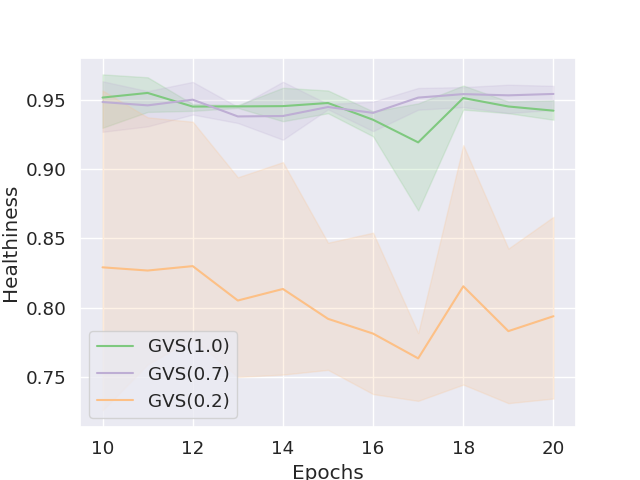
\includegraphics[width=0.25\textwidth]{./figs/healthiness.png}\label{fig31}}\subfigure[Dice curve (lr=0.0001)]{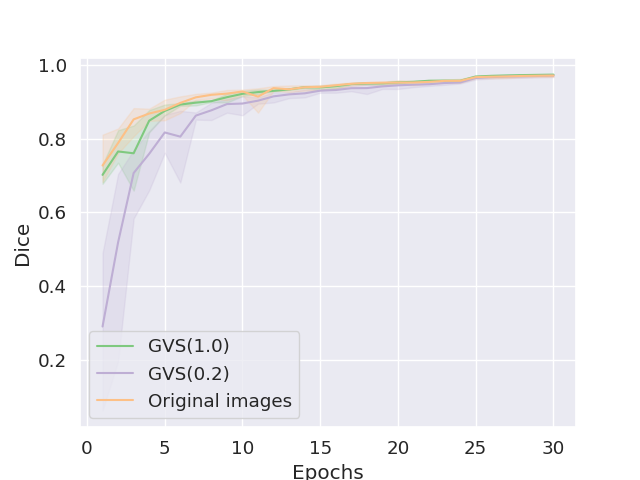
\includegraphics[width=0.25\textwidth]{./figs/hm_o.png}\label{fig32}}\subfigure[Dice curve (lr=0.1)]{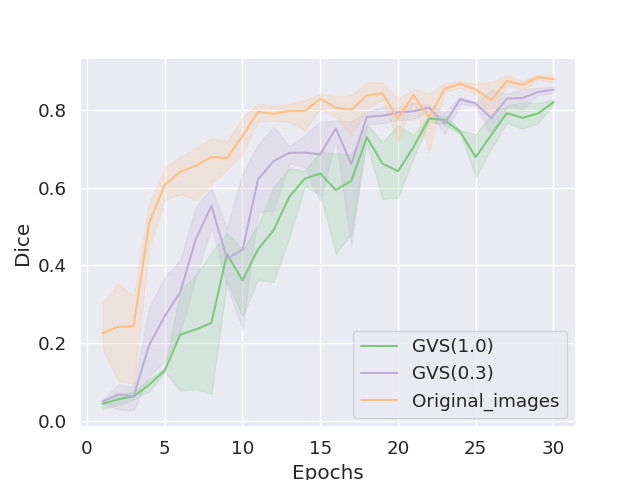
\includegraphics[width=0.25\textwidth]{./figs/hm.png}\label{fig33}}\subfigure[A-Dice]{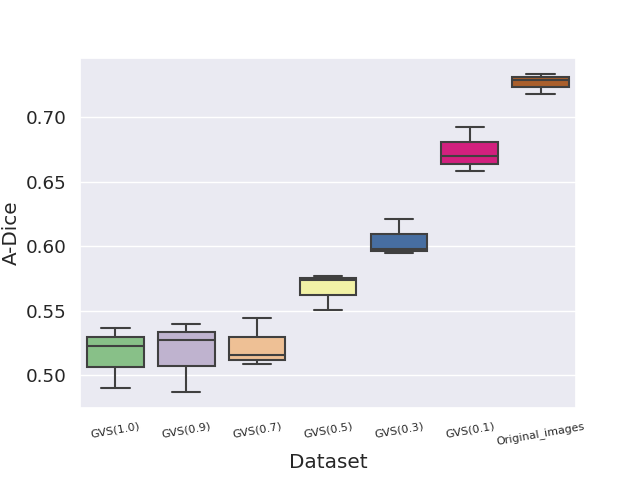
\includegraphics[width=0.25\textwidth]{./figs/hm3.png}\label{fig34}}
	\caption{(a) The "Healthiness" proposed in literature \cite{xia2020pseudo} at various epochs. (b) The dice scores on the training data at each epoch when the segmentor is trained with $lr=0.0001$. (c)  The dice scores on the training data at each epoch when the segmentor is trained with $lr=0.1$. (d) The A-Dice evaluated on different synthetic images. Here, the GVS(1.0) represents the synthetic images generated by GVS which is trained using $100\%$ of training data. The GVS(0.1), GVS(0.2), GVS(0.3), GVS(0.5), and GVS(0.7) also can be deduced from this. Obviously, the GVS($a$) have more healthy appearances than GVS(b) when $a>b$.}\label{fig3}
\end{figure*}

\subsection{Lesion contrast enhancement}
\label{subsection:enhancement}
It is well-known that the low contrast is an intrinsic nature of medical images and hinders tissue segmentation. Image enhancement, as one of the effective pre-processing techniques to tackle this problem, has been widely applied in medical image segmentation tasks \cite{vasuki2017survey}. 

Recently, Hamghalam et al. \cite{hamghalam2020high} confirmed the truth that increasing the contrast within underlying tissues can effectively improve the generalization ability of segmentation task in BraTS dataset. Inspired by this, we apply the proposed GVS to enhancing the contrast between tumors and normal tissues and then utilize the enhanced images to improve segmentation performance. 
%First, we extract the pathological information in the image space as follows
%\begin{equation}
%	R =  \left\{
%	\begin{array}{rcl}
%		x_s - x_p,       &      & x_s - x_p > T,\\
%		0,       &      & \text{Otherwise},
%	\end{array} \right.
%\end{equation} 
%where $R$ is the difference map between the pathological and synthetic image. To mitigate the potential impact of the weak residual signal on the generalization ability of segmentation task, we filter the smaller value in $R$. Then, we add the difference map into the input to enhance the contrast between normal tissue and lesions.
The process can be simply formulated as:
\begin{equation}
	x_{en} = x_p + \alpha * (x_s - x_p),
\end{equation} 
where $\alpha$ represents the degree of enhancement. We report a part of enhanced results in Figure \ref{fig5}. Intuitively, it is easier to distinguish tumors after enhancement. Next, we utilize the enhanced images to train the segmentor, which keeps consistent with the existing training pipeline. 








\section{Measuring Healthiness} \label{sec4}
Before presenting our metric, we first analyse the "Healthiness" metric proposed by Xia et al. \cite{xia2020pseudo}. To evaluate the healthiness, they first pre-trained a segmentor to estimate pathology from images. Then they used this segmentor to assess pathology from the synthetic images and checked how large the estimated pathology areas are. For more implementation details, we recommend reading Sec 4.4 in literature \cite{xia2020pseudo}. This process sounds reasonable but still exists the following shortcomings. First, the pre-trained segmentor is vulnerable to the artifacts both far away from both pathological and healthy regions in the distributional space. Thus, under these circumstances, this metric cannot accurately assess how healthy the synthetic images are. For example, the counterfeit images in Figure \ref{fig62} are obviously abnormal. However, the pre-trained segmentor cannot recognize the abnormalities entirely, and further results in false high performance. Second, this metric cannot quantitatively and even qualitatively reflect the healthiness of synthetic images. We repeatedly pre-trained three segmentors and then used them to calculate the metrics on the same synthetic images. As shown in Figure \ref{fig31}, the results at various epochs and runtimes, especially in the case of GVS(0.2), fluctuate drastically. Another phenomenon is that the performance of the GVS(0.7) may surpass the GVS(1.0) at some epochs, which is unreasonable since the model trained on more data is certainly superior to that trained on fewer data. These phenomenons imply that the model selection greatly affects the quantitative and qualitative results.

%\begin{figure}
%	\centering
%	\subfigure[Input]{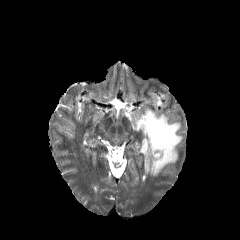
\includegraphics[width=0.24\columnwidth]{./figs/82_img1.jpg}\label{fig61}}
%	\subfigure[Counterfeit image]{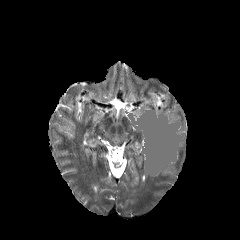
\includegraphics[width=0.24\columnwidth]{./figs/82_img2.jpg}\label{fig62}}
%	\subfigure[Prediction]{
\includegraphics[width=0.24\columnwidth]{./figs/82_pred2.jpg}\label{fig65}}
%	\subfigure[Label]{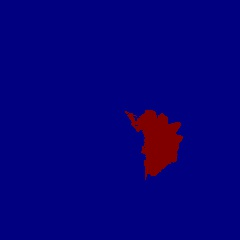
\includegraphics[width=0.24\columnwidth]{./figs/82_label.jpg}\label{fig64}}
%	\subfigure[Input]{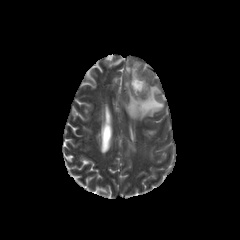
\includegraphics[width=0.24\columnwidth]{./figs/22_img1.jpg}\label{fig65}}
%	\subfigure[Counterfeit image]{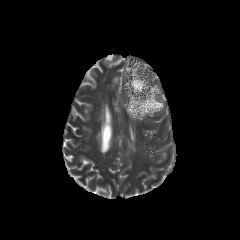
\includegraphics[width=0.24\columnwidth]{./figs/22_img2.jpg}\label{fig66}}
%	\subfigure[Prediction]{
\includegraphics[width=0.24\columnwidth]{./figs/22_pred2.jpg}\label{fig67}}
%	\subfigure[Label]{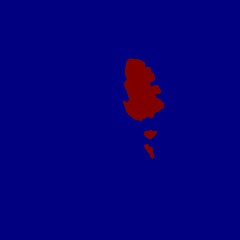
\includegraphics[width=0.24\columnwidth]{./figs/22_label.jpg}\label{fig68}}
%	\caption{The results of pre-trained segmentor evaluated on two different type of counterfeit images. The columns from left to right respectively represent input, counterfeit image, the prediction of counterfeit image, and lesion annotation. Two rows respectively inject two different artifacts. The counterfeit image in the first row is generated by filling the pathological regions with the average value of normal ones. The second row adds the gaussian noise with zero mean and 0.2 covariance in the pathological regions.}\label{fig6}
%\end{figure}

\begin{figure}
	\centering
	\subfigure[Inputs]{\begin{minipage}[b]{0.25\linewidth} 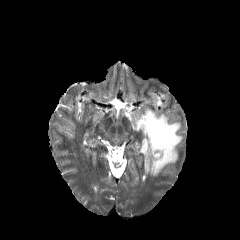
\includegraphics[width=\linewidth]{./figs/82_img1.jpg}\vspace{1pt} 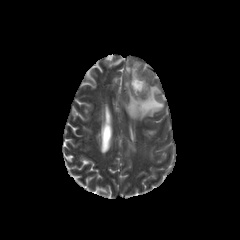
\includegraphics[width=\linewidth]{./figs/22_img1.jpg}\vspace{1pt}\end{minipage}\label{fig61}}\subfigure[Counterfeit images]{\begin{minipage}[b]{0.25\linewidth} 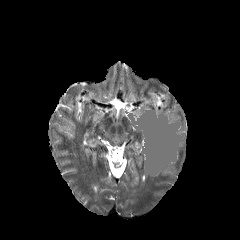
\includegraphics[width=\linewidth]{./figs/82_img2.jpg}\vspace{1pt} 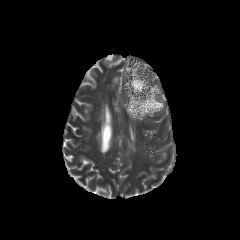
\includegraphics[width=\linewidth]{./figs/22_img2.jpg}\vspace{1pt}\end{minipage}\label{fig62}}\subfigure[Predictions]{\begin{minipage}[b]{0.25\linewidth} 
\includegraphics[width=\linewidth]{./figs/82_pred2.jpg}\vspace{1pt} 
\includegraphics[width=\linewidth]{./figs/22_pred2.jpg}\vspace{1pt}\end{minipage}\label{fig63}}\subfigure[Labels]{\begin{minipage}[b]{0.25\linewidth} 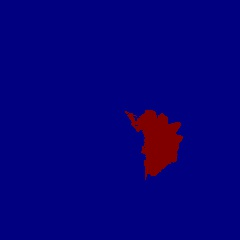
\includegraphics[width=\linewidth]{./figs/82_label.jpg}\vspace{1pt} 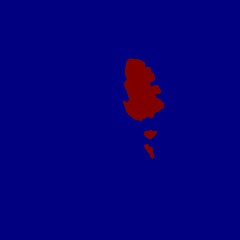
\includegraphics[width=\linewidth]{./figs/22_label.jpg}\vspace{1pt}\end{minipage}\label{fig64}}
	\caption{The results of pre-trained segmentor evaluated on two different type of counterfeit images. The images from left to right respectively represent input, counterfeit image, the prediction of counterfeit image, and lesion annotation. Two rows respectively inject two different artifacts. The counterfeit image in the first row is generated by filling the pathological regions with the average value of normal tissues. The second row adds the gaussian noise with zero mean and 0.2 covariance in the pathological regions.}\label{fig6}
\end{figure}

Our metric is inspired by the study of label noise. Zhang et al. \cite{zhang2016understanding} revealed an interesting phenomenon that training data with false/noisy labels requires more time to be fitted by the network. Similar to this, aligning well-transformed pixels (i.e., these pixels can be viewed as healthy ones) and original lesion annotations is counterfactual and hampers the fitting/convergence. To verify this, we utilize healthy or synthetic data (e.g., healthy images, synthetic images generated by GVS(1.0) and GVS(0.2)) to train a segmentor and then assessed the convergence speed by plotting the dice scores on the training data at various epochs. The results are shown in Figure \ref{fig32}, and we discovered that three models finally attain similar dice values but have different convergence speeds. The model trained on healthy images achieves the fastest convergence speed, followed by GVS(0.2) and GVS(1.0).

We further carefully observe the dice curves in Figure \ref{fig32} and find two disadvantages for quantitatively analyzing healthiness. 1) The models trained on GVS(0.2), GVS(1.0), and original images attain similar performances, which implies that this curve has lower discriminability for images with varying degrees of healthiness. 2) The performances at initial epochs are unstable and may mislead final results. To tackle the first disadvantage, we further utilize another property of false/noisy labels. That is, the higher learning rate will suppress the memorization ability of the DNN and prevents it from fitting labels \cite{Tanaka2018JointOF}. Thus, Simply improving the learning rate (i.e., from 0.0001 to 0.1) can obtain the results presented in Figure \ref{fig33}. We find that the difference of convergence speed for the three types of images is magnified significantly. For the second disadvantage, we design the ensemble strategy to improve the stability. To sum up, we propose a new metric to evaluate the convergence speed by averaging the dices at multi epochs (A-Dice), that can be formulated by
\begin{equation}
	\text{A-Dice} = \frac{1}{E}\sum_{e=1}^{E} dice_e,
\end{equation} 
where $E$ denotes the total epochs, and $dice_e$ represents the dice evaluated on the training data after the $e$-th epoch. Note that the lower A-Dice denotes faster convergence speed and further represents more healthy appearances.

We further stress why the proposed A-Dice can alleviate the shortcoming existing in the "Healthiness". First, any artifact is distributional different from the normal tissues and can be quickly fitted by the segmentor. As a result, it will be judged as unhealthy due to fast convergence. Second, although the dice at each epoch may be unstable, A-Dice can decrease deviation by averaging the dices at multi epochs.

To confirm the stability and reliability of A-Dice, we present the A-Dice of seven types of images, GVS(1.0), GVS(0.9), GVS(0.7), GVS(0.5), GVS(0.3), GVS(0.1), and original images, in Figure \ref{fig34} and provide qualitative analysis for them. First, for the same image, the fluctuation range of A-Dice is about 0.05 and is less than "Hwealthiness" \cite{xia2020pseudo} and subjective evaluation (rf. Table \ref{tab2}). Second, A-Dice accurately reflects the correct relative order for different synthetic images. That is, the A-Dice of GVS(a) is smaller than GVS(b) when $a>b$. Furthermore, we find A-Dice agrees with the subjective evaluation to a certain extent. That is, the PHS-GAN and ANT-GAN achieve close results for A-Dice (0.607 and 0.618, rf. Table \ref{tab1}), which also happens to the subjective metric, "Healthiness" (3.800 and 3.803, rf. Table \ref{tab2}). This also confirms the reliability of A-Dice.

\section{Experiments} \label{sec5}
\subsection{Datasets}
We validate our method on two widely-used public datasets: Multimodal Brain Tumor Segmentation Challenge 2019 dataset (BraTS19) \cite{menze2014multimodal,bakas2017advancing} and Liver Tumor Segmentation Challenge dataset (LiTS) \cite{bilic2019liver}.

\noindent\textbf{BraTS.} We use the training set of BraTS, which contains 259 GBM (i.e., glioblastoma)  and 76 LGG (i.e., lower-grade glioma) volumes that have been skull-stripped, interpolated to an isotropic spacing of $1mm^3$ and co-registered to the same anatomical template. Each volume includes 4 modalities (i.e., T1, T2, T1c, and Flair), and the slice is $240\times240$. We make use of the T2 of GBM, and split them into training (234 volumes) and test sets (25 volumes). For each volume, we clip the intensities to $[0, V_{99.5}]$, where $V_{99.5}$ is the $99.5\%$ largest pixel value of the corresponding volume.

\noindent \textbf{LiTS.} We use the training data set of LiTS, which contains 131 CT scans of the liver acquired from 7 different clinical institutions. The resolution of the slice is $512\times512$.  We divide the datasets into training (118 scans) and test set (13 scans). We truncate the image intensity values of all scans to the range of $[-200,250]$ to remove the irrelevant details \cite{li2018h}.

\subsection{Implementation details}
The generator and the segmentor respectively adopt the encoder-decoder \cite{Johnson2016PerceptualLF}  and U-Net \cite{ronneberger2015u} architectures. We implement the proposed method based on Pytorch. We employ a poly learning rate policy where the initial learning rate is multiplied by $(1-\frac{epoch}{total\_epoch})^{0.8}$ after each epoch. The base learning rate is set to $0.001$, and the $E$ is set to $20$. The optimizer is Adam with $\beta_1 = 0.9$, $\beta_2 = 0.99$. Batchsize is set to 8 for BraTS and 4 for LiTS. $\lambda$ to balance the healthiness and identity is set $10.0$.  The training is implemented on an NVIDIA TITAN XP GPU.

\subsection{Baselines}
We compare our method with the following three approaches:

\noindent\textbf{VA-GAN.} The architecture of VA-GAN \cite{baumgartner2018visual} contains a generator and discriminator that are alternatively updated to generate pseudo healthy images. Furthermore, the VA-GAN introduces the $\mathcal{L}_1$ loss to minimize the difference between the synthetic and pathological images. We use the official code\footnote{https://github.com/baumgach/vagan-code
} and train it on our dataset.

\noindent\textbf{ANT-GAN.}  The ANT-GAN \cite{sun2020adversarial} is a variant of the Cycle-GAN. In comparison with the Cycle-GAN, it adds the $\mathcal{L}_2$ loss between the pathological and synthetic images to maintain the normal tissue and add a shortcut in the process of transforming the pathological images into healthy ones to simplify the task.

\noindent\textbf{PHS-GAN.} The PHS-GAN \cite{sun2020adversarial} also is a variant of the Cycle-GAN. To address the one-to-many problem for Cycle-GAN, the PHS-GAN estimates a disease map from a pathological image using a segmentation network and then uses the map to provide information about disease location. We also use the official implementation\footnote{https://github.com/xiat0616/pseudo-healthy-synthesis}.

\subsection{Other evaluation metrics}
To comprehensively assess the effectiveness of our method, synthetic images are evaluated from the aspects of healthiness and subject identity objectively and subjectively. Next, we respectively introduce these metrics in detail.

\noindent\textbf{Objective metrics.} The overall quality of pseudo-healthy images consists of healthiness and subject identity.  In Section \ref{sec4}, we have described the proposed metric A-Dice that can assess the healthiness of pseudo-healthy images. Here, we then introduce how to measure the subject identity, which can be expressed as calculating the visual similarity of normal tissue between pathological and synthetic images. The common metrics to achieve this goal are SSIM and PSNR. We adopt both of them since they have respective advantages and limitations in practice \cite{hore2010image}.

\noindent\textbf{Subjective metrics.}  Subjective metric is the gold standard to evaluate the quality of pseudo-healthy images. Thus, we adopt the human evaluation methods similar to \cite{xia2020pseudo}. Keeping the same with objective metrics, the human evaluation also is composed of the factors of healthiness and subject identity. The detailed process of subjective testing is presented as follows.

We randomly select 100 synthetic outputs of all comparison methods and arranged them as follows. Except for the pathological input placed in the first position, the synthetic outputs of all comparison methods are randomly arranged in the next four positions. The last position is occupied by the lesion annotation to better convey the pathological information to raters. Meanwhile, the raters are blinded to which algorithm generated each image. The subjective ratings are rated on a five-level scale: 5 (excellent), 4 (good), 3 (fair), 2 (poor), and 1 (bad), and three medical image analysis researchers are asked to independently score each synthetic image from the aspects of healthiness (i.e., the scores from 5 to 1 represent that the healthiness declines sequentially) and subject identity (i.e., the scores from 5 to 1 represent that the subject identity is erased sequentially). 

\begin{figure}[htbp]
	\centering
	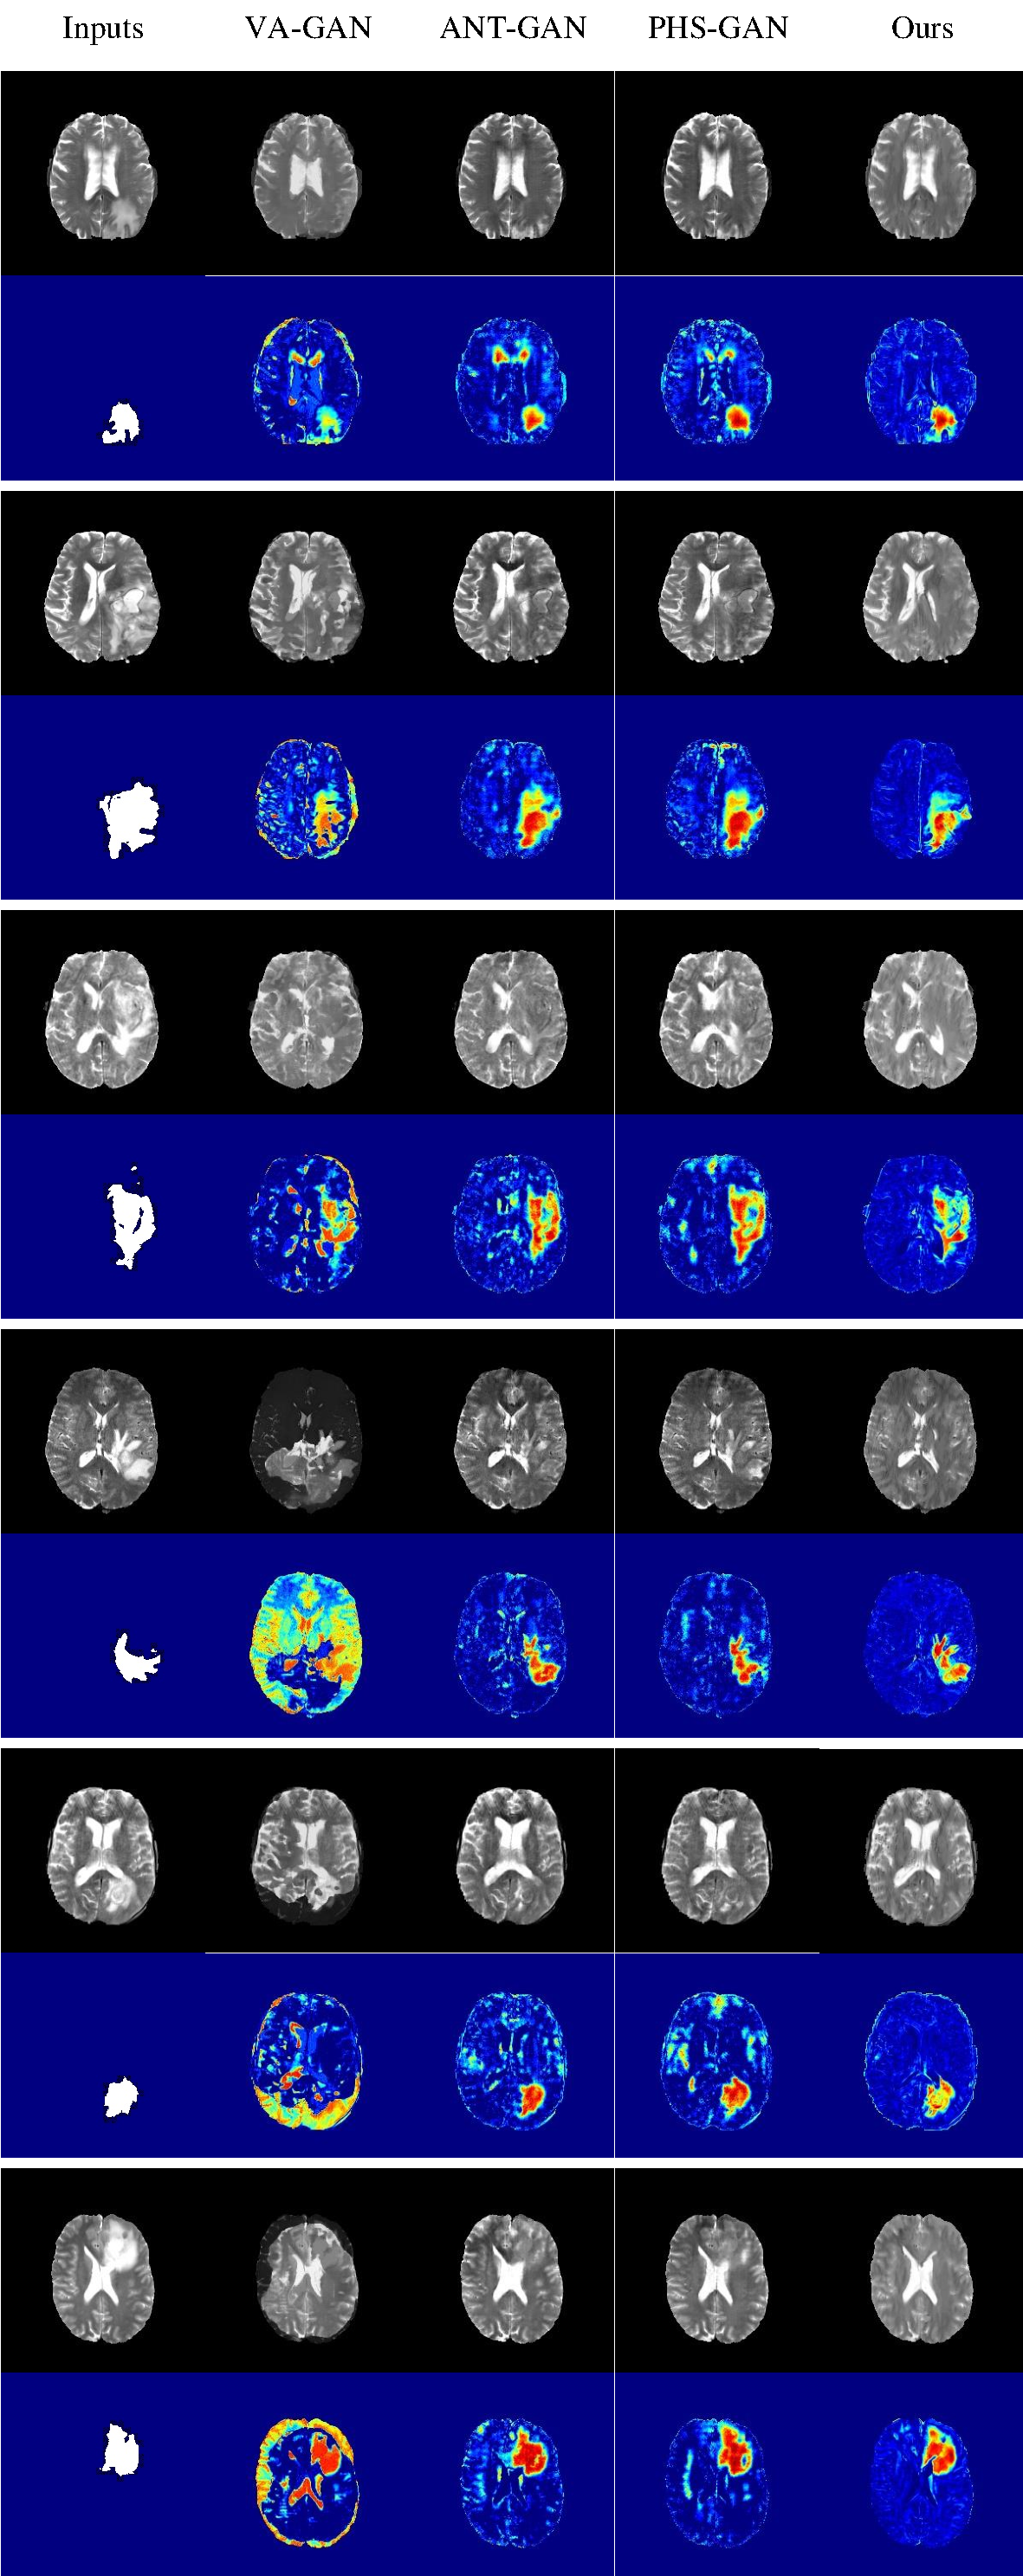
\includegraphics[width=\columnwidth]{./figs/results.pdf}
	\caption{Quantitative results on BraTS dataset. We plot six examples (blocks) from top to bottom. In each block, the first row show the input, synthetic images generated by VA-GAN, ANT-GAN, PHS-GAN and GVS. The second row show the lesion annotation and corresponding difference maps.}
	\label{fig7}
\end{figure}

\begin{figure*}
	\centering
	\subfigure[]{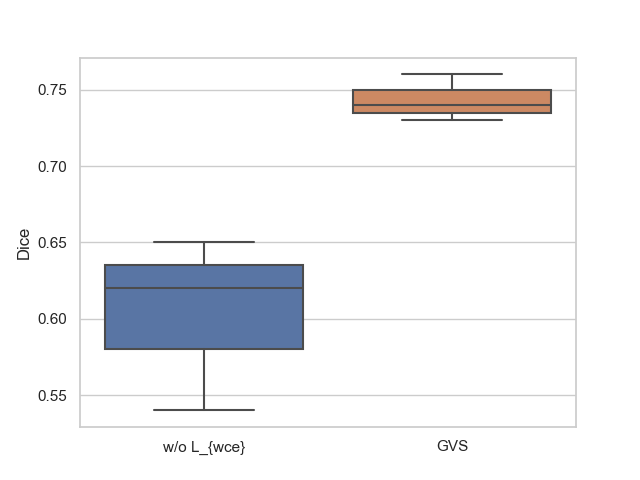
\includegraphics[width=0.25\textwidth]{./figs/Fig20.png}\label{fig91}}\subfigure[]{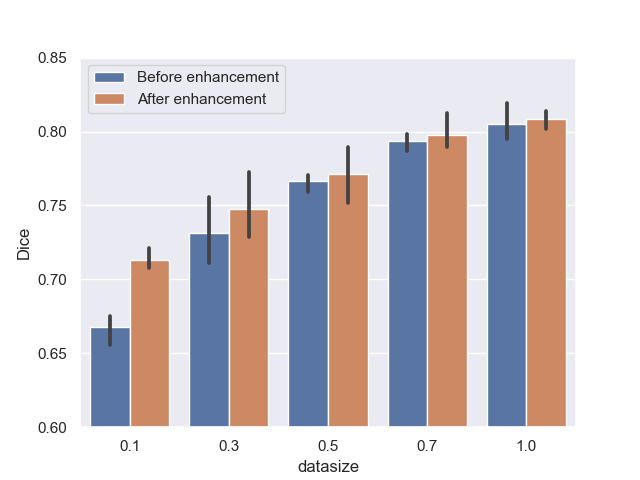
\includegraphics[width=0.25\textwidth]{./figs/enhancement_diff_datasize.png}\label{fig92}}\subfigure[]{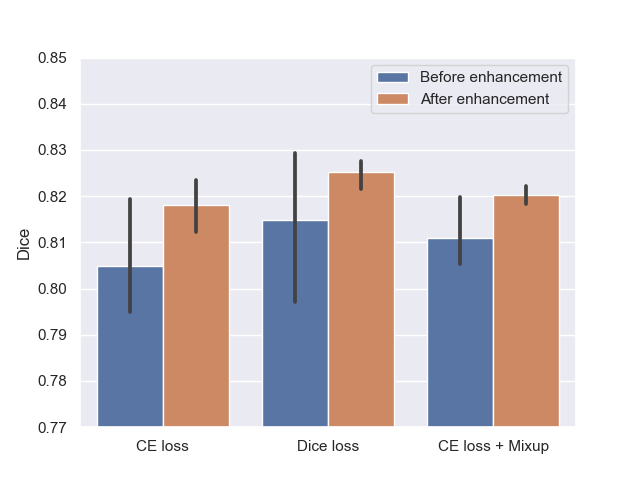
\includegraphics[width=0.25\textwidth]{./figs/compatibility.png}\label{fig93}}\subfigure[]{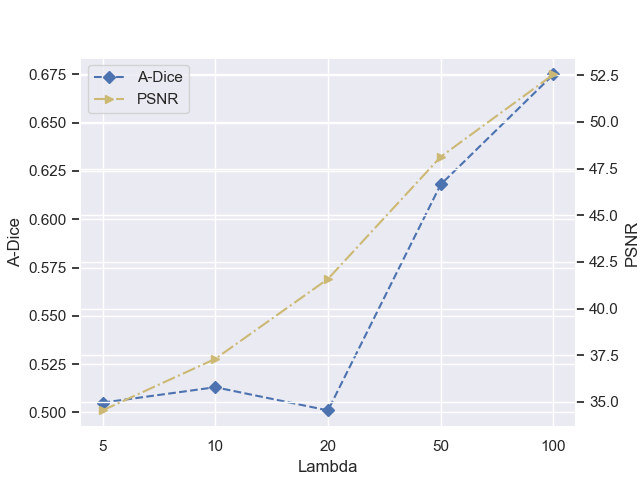
\includegraphics[width=0.25\textwidth]{./figs/sensitivity.png}\label{fig94}}
	\caption{(a) The generalization ability of the segmentor in the GVS. (b) The variety of segmentation performance before and after enhancement. (c) The variety of segmentation performance when combining with Dice loss and mixup. (d) The sensitivity analysis for $\lambda$.}
	\label{fig9}
\end{figure*}

\subsection{Comparison with State-of-the-art Methods} \label{sec55}
\noindent\textbf{Qualitative results.} The qualitative results are shown in Figure \ref{fig7}. The effectiveness of the methods is evaluated based on the identity and healthiness of synthetic images.

The "healthiness" can be judged by comparing whether pathological and normal regions are harmonious. If the pathological regions are in harmony with the normal ones in the synthetic images, such images are healthy. On the contrary, the pathological regions can be easily distinguished from the normal ones in the synthetic images, such images are viewed as being "no healthy". The performance of the VA-GAN fluctuates substantially. Some of the synthetic images have superior performance (e.g., the first and third examples in Figure \ref{fig7}). However, the major of them can be easily distinguished from the healthy images due to the poor reconstruction. The PHS-GAN and ANT-GAN removes most of the lesions, but some artifacts still existed (rf. the second, fourth, sixth samples in Figure \ref{fig7}). Finally, the proposed GVS removes most lesions and replaces them with a relatively healthy-like area.

The identity is determined by comparing the inputs and synthetic images in terms of structural details, brightness, contrast, and so on. Since the ANT-GAN, PHS-GAN, and the proposed GVS reconstruct the normal tissue accurately, we plot the difference maps between the inputs and synthetic images to magnify the differences. Combining the difference maps and labels, the proposed method achieves reconstruction of much higher quality than the other methods due to preserving more details of the brain tissues. It is noteworthy to mention that the cerebrospinal fluid had pixels with high intensities and is close to lesions. These regions are weakened by varying degrees by the other methods, whereas they are well-preserved by the proposed method. Overall, the VA-GAN could not keep the identity and lost a part of the lesion region in some cases. The PHS-GAN and ANT-GAN preserve the brain region but lost some details. Among all the methods, the proposed method achieves the best performance.


\begin{table}
	\centering
	\caption{Quantitative results on BraTS dataset. We report the average value and standard deviation of 3 trials.}	
	\begin{tabular}{llll}
		\toprule
		Method & SSIM $\uparrow$ & PSNR $\uparrow$ & A-Dice $\downarrow$ \\
		\midrule
		Original images & - & - & 0.736($\pm$0.310) \\
		VA-GAN \cite{baumgartner2018visual}  & 21.89($\pm$1.02) & 0.742($\pm$0.470) & - \\
		PHS-GAN \cite{xia2020pseudo} & 29.51($\pm$0.47) & 0.966($\pm$0.025) & 0.607($\pm$0.056) \\
		ANT-GAN \cite{sun2020adversarial} & 28.75($\pm$0.51) & 0.963($\pm$0.018) & 0.618($\pm$0.066) \\
		GVS(0.3) & \textbf{38.79($\pm$0.39)} & \textbf{0.995($\pm$0.013)} & 0.615($\pm$0.040) \\
		GVS w/o $\mathcal{L}_{wce}$ &  37.31($\pm$0.34) & 0.991($\pm$0.012) & 0.549($\pm$0.045) \\
		\rowcolor{gray!20} GVS(1.0) & 37.31($\pm$0.34) & 0.991($\pm$0.012) & \textbf{0.512($\pm$0.035)} \\
		\bottomrule
	\end{tabular}
	\label{tab1}
\end{table}


\noindent\textbf{Objective evaluation.} The quantitative results on the BraTS dataset are shown in Table \ref{tab1}. The results of SSIM and PSNR show that, in comparison to the VA-GAN, the other methods improve the visual similarity to a large extent since they utilize lesion annotations. The proposed method further improves the visual similarity compared to the other methods. As for the healthiness results, since the VA-GAN could not reconstruct the normal tissue, as shown in Figure \ref{fig7}), its A-Dice value is meaningless. Therefore, it is not considered. The values of $\mathbb{S}_{dice}$ of the ANT-GAN and PHS-GAN are similar, 0.618 and 0.607. In comparison to the original images, they decline by 0.118 and 0.129, respectively. The A-Dice value of the proposed GVS is 0.512. Compared to the existing methods, it attains substantial improvement. From another angle, only trained on 30 percent of training data, the GVS achieves the notable performance, where the A-Dice is close to the ANT-GAN and PHS-GAN while the SSIM and PSNR significantly exceed the existing methods. 



\begin{table}
	\centering
	\caption{Subjective evaluation on BraTS dataset. We report the average value and standard deviation of 3 raters.}	
	\begin{tabular}{lcc}
		\toprule
		Method & "Healthiness" $\uparrow$ & "Subject identity" $\uparrow$ \\
		\midrule
		VA-GAN \cite{baumgartner2018visual}  & 2.103($\pm$0.414) & 1.943($\pm$0.519) \\
		PHS-GAN \cite{xia2020pseudo} & 3.667($\pm$0.824) & 3.800($\pm$0.568) \\
		ANT-GAN \cite{sun2020adversarial} & 3.707($\pm$0.823) & 3.803($\pm$0.518) \\
		\rowcolor{gray!20} Our GVS & \textbf{4.457($\pm$0.330)} & \textbf{4.390($\pm$0.491)} \\
		\bottomrule
	\end{tabular}
	\label{tab2}
\end{table}

\begin{figure*}[htbp]
	\centering
	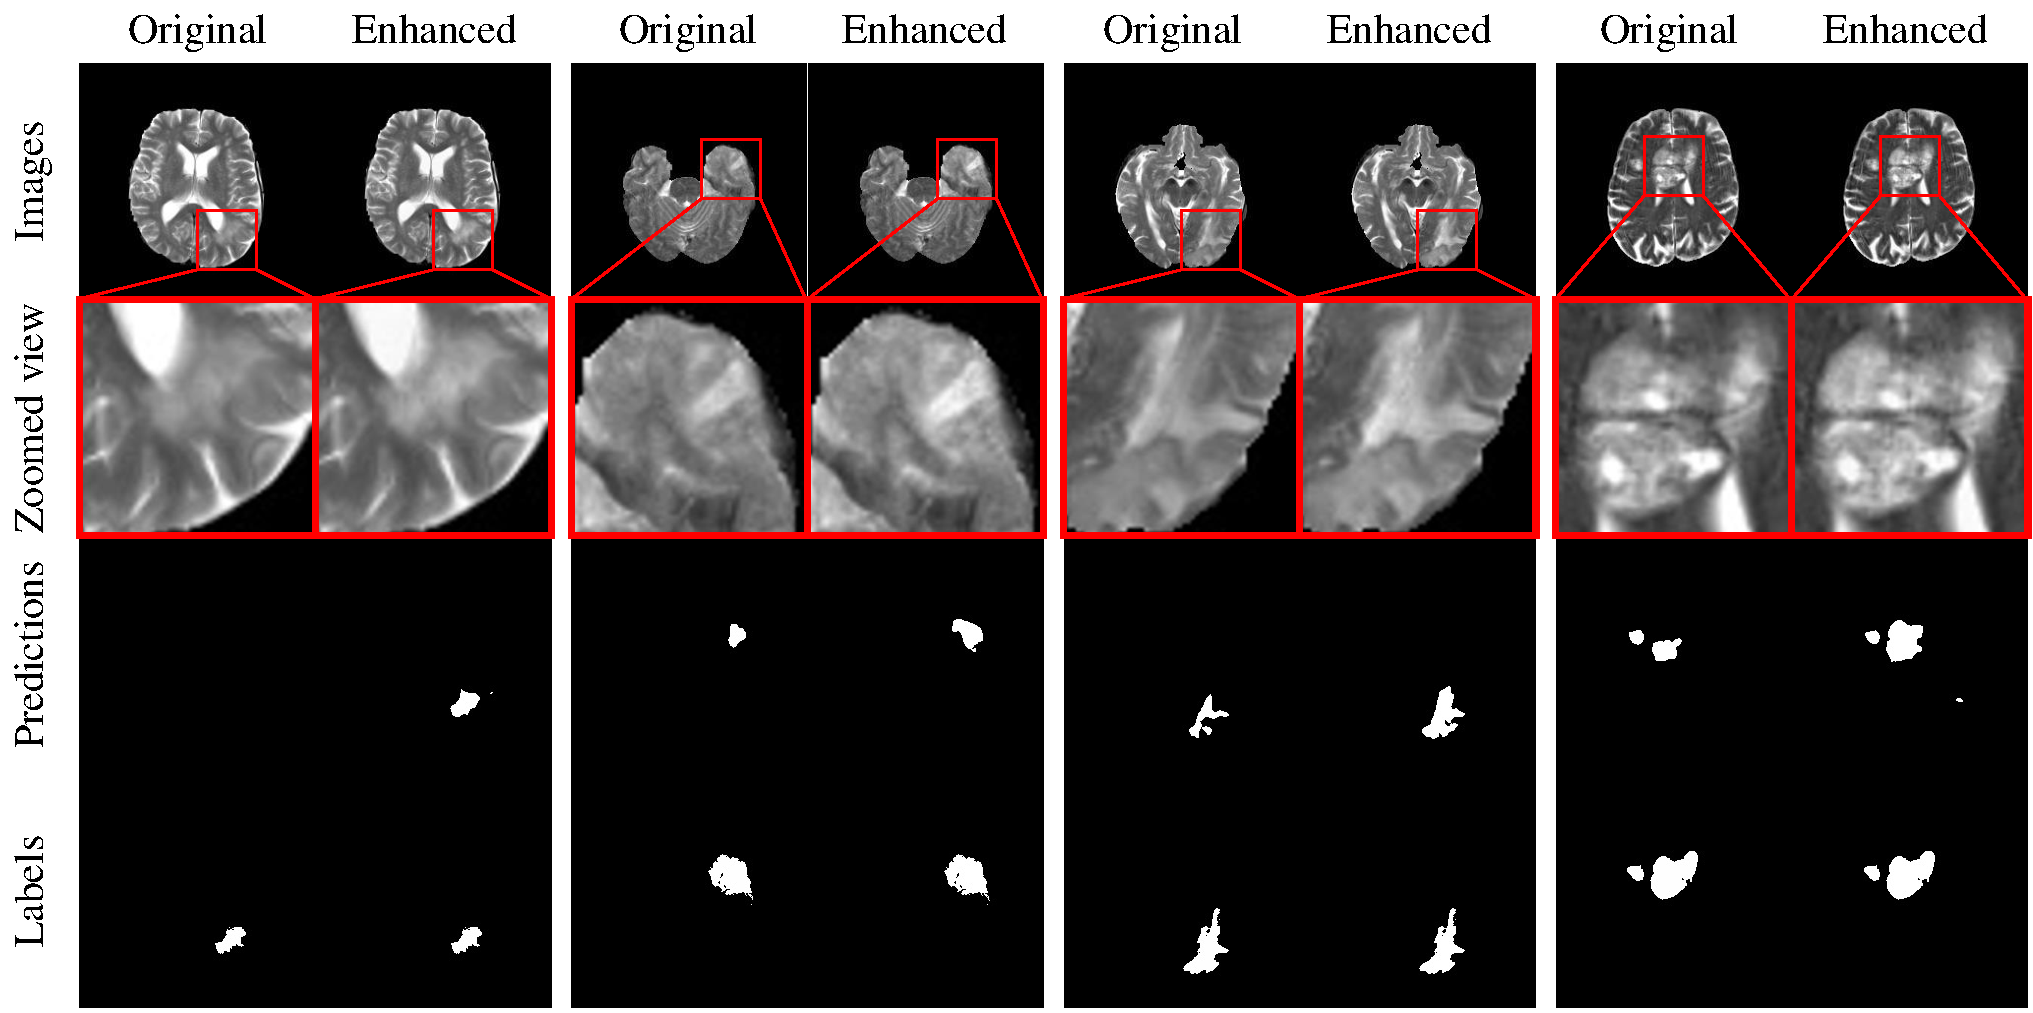
\includegraphics[width=\textwidth]{./figs/enhanced.pdf}
	\caption{Examples of segmentation predictions for enhanced results on BraTS dataset. Note that these results are generated when $\alpha=0.3$.}
	\label{fig8}
\end{figure*}


\begin{table*}
	\centering
	\caption{Comparison of the segmentation performances in the case of different $\alpha$. All results are averaged over 3 trials. Note that $\alpha = 0.0$ represents the images without enhancement, and the values in brackets are calculated by comparing the segmentation performances before or after enhancement. Max improvement is denoted in \textbf{bold}, and the second one is denoted in \underline{underline}.}
	\begin{tabularx}{400pt}{c *7{>{\Centering}X}}\toprule
		\multirow{2}{*}{BraTS} & $\alpha$ & 0.0 & 0.3 & 0.5 & 0.7 & 1.0 \\
		\cmidrule(l){2-7}
		~ & Dice & 0.805 & \underline{0.813(+0.008)} & 0.812(+0.007) & \textbf{0.818(+0.013)} & 0.808(+0.003) \\
		\midrule
		\multirow{2}{*}{LiTS} & $\alpha$ & 0.0 & 0.3 & 0.5 & 0.7 & 1.0 \\
		\cmidrule(l){2-7}
		~ & Dice & 0.643 & 0.655(+0.012) & 0.653(+0.010) & \textbf{0.666(+0.023)} & \underline{0.665(+0.022)} \\
		\bottomrule
	\end{tabularx}
	\label{tab3}
\end{table*}

\noindent\textbf{Subjective evaluation.} We report the subjective results in Table \ref{tab2}. The overall tendency of subjective results is similar to the objective ones. That is, the GVS shows the best performance. Subsequently, the PHS-GAN and ANT-GAN have similar results. Finally, the VA-GAN occupies the bottom position. Particularly, the performance difference between different methods are magnified, and our GVS has a more obvious performance advantage than other methods in the aspects of both "Healthiness" and "Subject identity". Furthermore, our GVS achieves near-ideal performance ("Healthiness": GVS (4.457) vs upper bound (5.0); "Subject identity": GVS (4.390) vs upper bound (5.0)), which suggest the near-perfect performance of the GVS from the expert perspective.



\subsection{Effectiveness of difference-aware loss} \label{sec56}
In Section \ref{subsection:segmentor}, we claim that the segmentor in the basic GVS has a poor generalization ability due to the mismatch between synthetic images and lesion annotations. As a result, the generator will be misguided and generate images with poor visual quality. We first evaluate the generalization ability of the segmentor before and after adding difference-aware loss. To this end, the pathological images are sent to the segmentor trained by the GVS and GVS w/o difference-aware loss, and then the corresponding dice scores are calculated. The results are shown in Figure \ref{fig91} and illuminate that the GVS achieves a higher average dice score and lower variance compared to the GVS w/o $\mathcal{L}_{wce}$, which confirms that the difference-aware loss could improve the generalization ability of the segmentor. 

Next, we further test and verify the effectiveness of difference-aware loss on the healthiness and subject identity of synthetic images. The results are shown in Table \ref{tab1}. We discover that the A-Dice has a significant improvement and the SSIM increases slightly, which implies a tight relationship between the generalization ability of the segmentor and the healthiness degree of synthetic images. 

%Furthermore, we extend the experiments by modifying the network structure and learning rate of segmentor to explore the relationship between the power of segmentor and synthetic images quality.


\subsection{Results on contrast-enhanced brain tumor segmentation} \label{sec57}
The segmentation performance after enhancement is shown in Table \ref{tab3}. We find that under different $\alpha$ the segmentation performance all have improvements to different extents. Next, we further explore the reason that may lead to performance improvement after enhancement by qualitative comparison. We show four examples with lower contrast in Figure \ref{fig9}. The results indicate that the enhancement highlights the lesions and eventually results in more accurate segmentation.

Then, we conduct the experiments to explore the improvements bringing from the enhancement under different data sizes. The results are shown in Figure \ref{fig92}, and we find that the improvements are more evident when the data size is smaller. We guess that this is because that the network is easy to overfit when data size is small and the enhancement explicitly regularizes the network at the image level so that better solutions are easier to be found.

Lastly, we combine the enhancement with other techniques (e.g., Dice loss and mixup) that can effectively improve segmentation performance to test and verify its compatibility with other techniques. Dice loss is presented in V-Net \cite{Milletari2016VNetFC} and is one of the most common loss functions used in medical image segmentation. Mixup \cite{zhang2017mixup} is an effective data augmentation technique in the classification task. Recently, it is also introduced in medical image segmentation \cite{eaton2018improving} and has been proven effective. The results are shown in Figure \ref{fig93}. We discover that these two techniques indeed improve the segmentation performance in brain tumor segmentation and our enhancement further improves the segmentation performance on their basis.


\subsection{Sensitivity analysis of $\lambda$} \label{sec58}
Our GVS only contains one hyperparameter $\lambda$, which is used to balance the power of the visual residual loss  $\mathcal{L}_R$ and adversarial loss $\mathcal{L}_{s2}$ when training the generator $G$. Here, we investigate the sensitivity of GVS for different choices of $\lambda$ and report the results in Figure \ref{fig8} (e). We discover that the "Healthiness" and "Subject identity" take up the opposite position. Better healthiness (lower A-Dice value) means worse subject identity and vise versa. Especially, when $\lambda \in [5, 20]$, the healthiness varies slightly. 


\begin{figure}
	\centering
	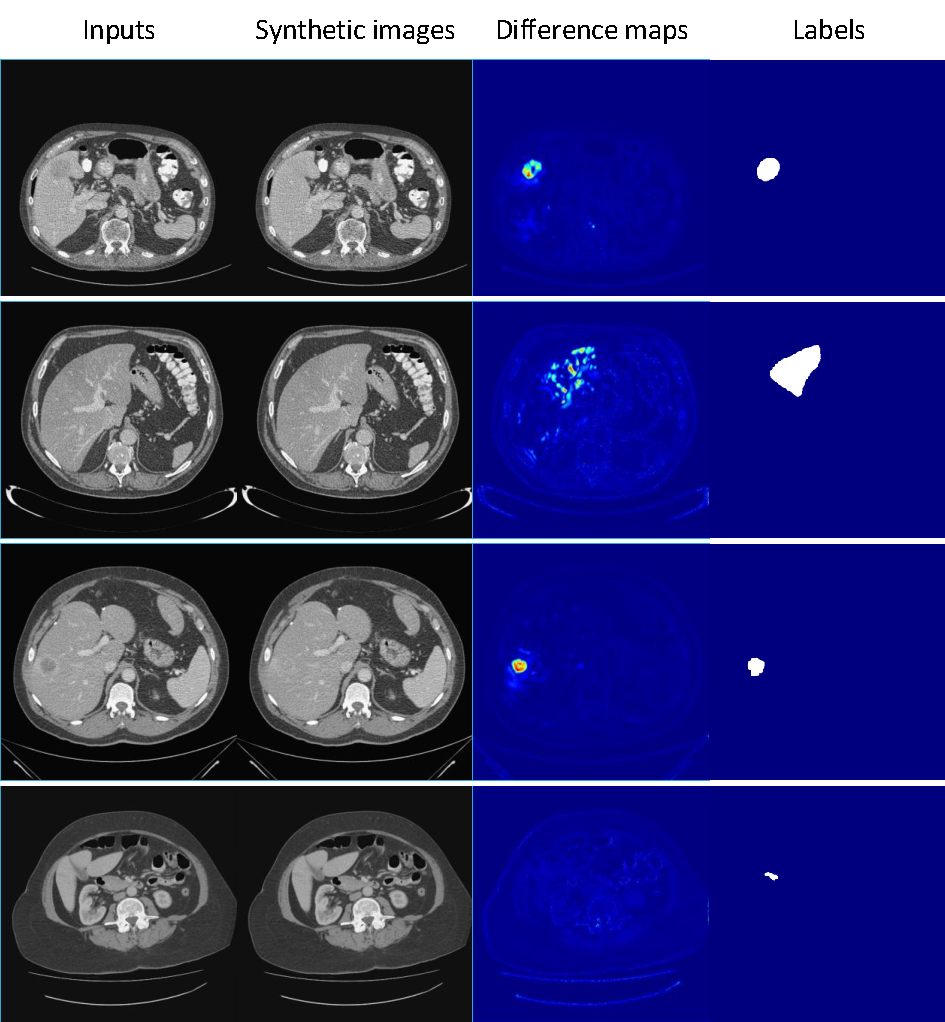
\includegraphics[width=\columnwidth]{./figs/result2.pdf}
	\caption{Quantitative results on LiTS dataset. We plot four examples (blocks) from top to bottom. In each block, the first row show the input, synthetic image, difference map, and label.}
	\label{fig10}
\end{figure}

\subsection{Expanded results on LiTS dataset} \label{sec59}
The proposed GVS is also evaluated on a public CT dataset, LiTS. The results are displayed in Figure \ref{fig10} and show that the proposed method determines the identity of images and transforms the high-contrast lesions well, as shown in the top row in Figure \ref{fig10}, but results corresponding to the images with lower-contrast are not satisfactory, as shown in the bottom row in Figure \ref{fig10}. This is because that the images in the LiTS dataset had higher resolution, and even more importantly, the lesions had smaller volumes and lower contrast. 

We also apply the synthetic results into contrast-enhanced segmentation, and the results are shown in Figure \ref{fig8} (f). We first find that the performance improvement is more significant than the BraTS. We conjuncture that it's owing to the contrast enhancement facilitates the segmentation more significantly in the case of lower-contrast. The phenomenon that higher $\alpha$ results in more improvement also confirms this view.


\section{Discussion and Conclusion} \label{sec6}
In this work, our efforts mainly include three parts. The first one is proposing an adversarial framework consisting of a generator and a segmentor to cope with the problem of pseudo-healthy synthesis.  

The experiments show that our GVS achieves excellent performance compared to state-of-the-art methods. Besides the results and analysis in Section \ref{sec55}, we further emphasize that the healthiness and subject identity are competing (shown in Section \ref{sec58}). A similar attribute, the contradiction between reconstruction and adversarial losses, also is verified in the GAN \cite{ramasinghe2020conditional}. Hence, achieving superior performance in the terms of both healthiness and subject identity for our GVS is impressive.

In the Section \ref{subsection:segmentor}, we design the difference-aware loss to alleviate the poor generalization ability of the segmentor, which is verified to be effective for improving the generalization ability of the segmentor and "Healthiness" of synthetic images (rf. Section \ref{sec56}). But we think this design is coarse and still has room for improvement. For example, we do not consider that at first epochs the synthesis is imperfect and the difference maps are less meaningful.   Hence, how to improve the difference-aware loss or design a novel scheme to enhance the generalization of the segmentor is our next target.

In Section \ref{sec56}, we reveal the tight relationship between the power of segmentor and the healthiness of synthetic images. Based on this, we further conjecture that strengthening the segmentor contributes to further improve the capacity of GVS. On the other hand, the family of 3D fully convolutional networks has become mainstream choices in the field of 3D medical image segmentation. Hence, we plan to upgrade the GVS with 3D structures to further improve synthetic performance. Furthermore, whether the obtained results can improve the segmentation performance of the 3D segmentor is also explorable.

The second part of the main work is using the disentangled pathological information in pseudo-healthy synthesis to enhance the contrast between normal tissue and lesions. The results in Section \ref{sec57} and \ref{sec59} illustrate that the enhancement technique based on GVS effectively improves the performance of the current segmentation model by enhancing contrast. Moreover, this technique has good compatibility with other techniques that are good for segmentation. Hence, it is able to improve segmentation performance as an extra trick. Last, but most important, the segmentor trained on less training data benefits more from the enhancement is an interesting and significant phenomenon. It is well known that training a model with a small dataset is a critical and challenging topic in medical image segmentation \cite{zhang2019survey}. The GVS may be one effective solution to deal with this problem and merits further exploration.

The third part is proposing a stable and reliable metric, A-Dice, to measure the healthiness of synthetic images. Furthermore, we think this metric has the potential to extend more applications. For example, we plan to use this metric to measure the pathological information in the images and explore the relationship between it with downstream tasks, such as tumor grading and survival prediction.

To sum up, the experimental results positively identify our claim in this paper. This may have a positive impact on the development of pseudo-healthy synthesis from the aspects of 1) improving the performance of pseudo-healthy synthesis, 2) developing one meaningful downstream task, and 3) proposing a novel metric with great reproducibility and discriminability to measure "Healthiness". On the other hand, we also think that the proposed GVS and A-Dice can associate with other medical image analysis tasks and deal with them from another perspective.

\bibliographystyle{IEEEtran}
\bibliography{GVS}

\end{document}
